\subsection{Etapa de análise}

\subsubsection{Lista de Requisitos x Funcionalidades}

\begin{longtable}[h!]{ | M{1cm} | T{2cm} | T{1.5cm} | T{4cm} | T{4cm} | } \hline

    \textbf{id. Req} & \textbf{Requisito} & \textbf{Ator} & \textbf{Funcionalidade} & \textbf{Regra de negócio} \\ [5pt] \hline
    
    1 & CRUD de receitas & Usuário & Criar nova receita & O sistema deve permitir o usuário criar novas receitas \\  \hline

    2 & CRUD de receitas & Usuário & Ler receitas & O sistema deve permitir o usuário ler receitas criadas \\  \hline

    3 & CRUD de receitas & Usuário & Atualizar receitas criadas & O sistema deve permitir o usuário atualizar receitas criadas \\  \hline

    4 & CRUD de receitas & Usuário & Deletar receitas criadas & O sistema deve permitir o usuário deletar receitas criadas \\  \hline

    5 & CRUD de despesas & Usuário & Criar nova despesa & O sistema deve permitir o usuário criar novas despesas \\  \hline

    6 & CRUD de despesas & Usuário & Ler despesa & O sistema deve permitir o usuário ler despesas criadas \\  \hline

    7 & CRUD de despesas & Usuário & Atualizar despesas criadas & O sistema deve permitir o usuário atualizar despesas criadas \\  \hline

    8 & CRUD de despesas & Usuário & Deletar despesas criadas & O sistema deve permitir o usuário deletar despesas criadas \\  \hline
    
    9 & Definir despesa recorrente & Usuário & Definir a recorrência da despesa & O sistema deve permitir o usuário definir a recorrência de uma despesa \\  \hline

    10 & Definir receita recorrente & Usuário & Definir a recorrência da receita & O sistema deve permitir o usuário definir a recorrência de uma receita \\  \hline

\end{longtable}


\subsubsection{Lista de Requisitos Não-Funcionais}

\begin{longtable}[h!]{ | M{1.5cm} | T{9cm} | l | } \hline

    \textbf{id. Req} & \textbf{Requisito} &\textbf{Categoria} \\ [5pt] \hline
    
    1 & Desenvolvimento do banco de dados deverá ser realizado em node.js & Performance \\  \hline

    2 & Desenvolvimento do backend deverá ser realizado em node.js & Performance \\  \hline

    3 & Desenvolvimento da interface de usuário deverá ser realizado  utilizando react & Performance \\  \hline

    4 & O compartilhamento do gerenciamento financeiro deve ser feito apenas com usuários especificados & Segurança \\  \hline

\end{longtable}

\subsubsection{Diagrama de Caso de Uso}
O diagrama de caso de uso foi realizado utilizando a o site \textit{draw.io}, o resultado pode ser observado na figura 1. 
\begin{figure}[h!]
    \centering
    \caption{Diagrama de caso de uso}
    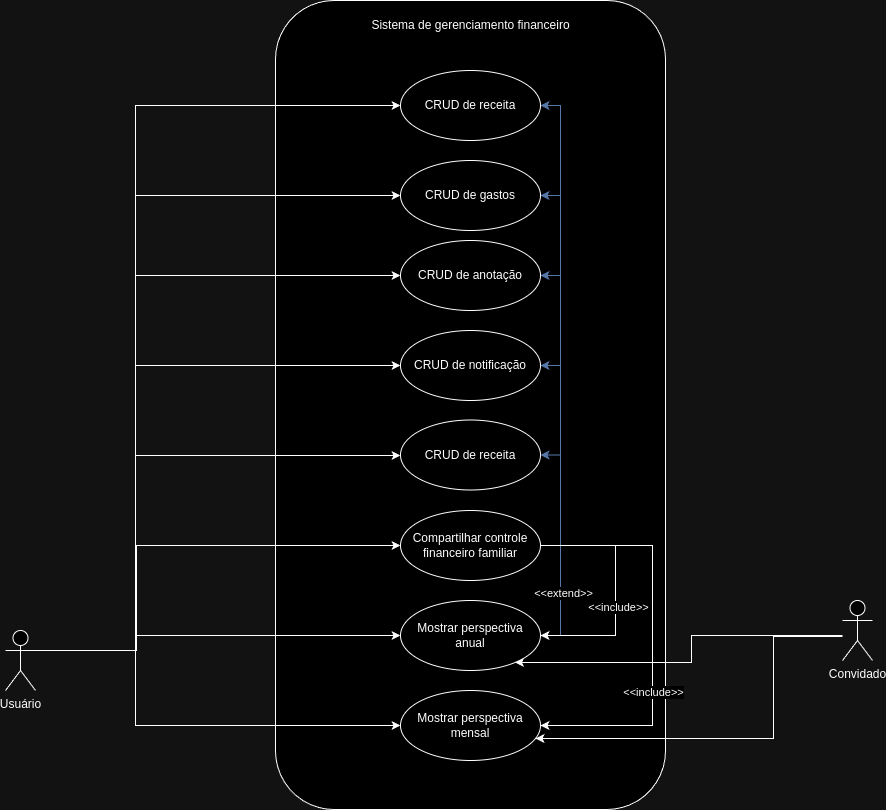
\includegraphics[scale=0.4]{images/money-tracker-Use-Case-Diagram.png}
\end{figure}

\subsubsection{Diagrama de Classe}
O diagrama de classes foi realizado utilizando a o site \textit{draw.io}, o resultado pode ser observado na figura 2. 

\begin{figure}[h!]
    \centering
    \caption{Diagrama de caso de classe}
    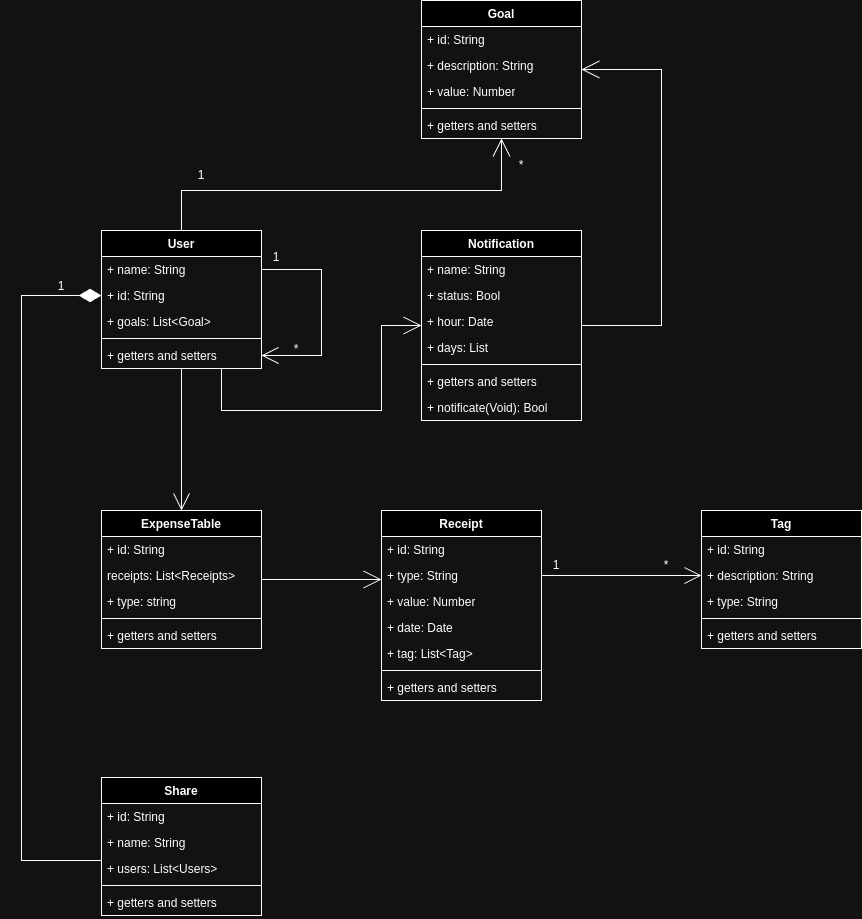
\includegraphics[scale=0.4]{images/money-tracker-Class-Diagram.png}
\end{figure}